% !TeX spellcheck = en_US
\section{Race Detection by Mining Locking Rules}
\label{sec_technique}
To address the above challenges, we propose three key techniques. For {\em C1}, 
we propose an {\em alias-aware rule mining method} to automatically deduce 
locking rules. For {\em C2}, we propose a {\em lock-usage analysis} to filter 
out false data races by validating concurrency of code paths. For {\em C3}, we 
propose a pattern-based estimation to extract harmful races that can trigger 
memory or logical bugs such as null-pointer dereference and data inconsistency. 
We introduce them as follows:

\subsection{Alias-Aware Rule Mining Method}
\label{subsec_rule_mining}
The relationship between variables and locks are not well documented in OS 
kernels, but it can be inferred from the kernel code. Specifically, a variable 
is often protected by the lock stored in the same data structure. And thus if a 
variable is accessed after acquiring a lock existing in the same data structure 
in most cases, it is likely to be protected by the lock. Whether a variable and 
the protecting lock exist in the same data structure can be determined though 
an alias graph~\cite{Li:ASPLOS22, Kastrinis:CC18} by finding their common 
ancestor. Based on this insight, we propose an {\em alias-aware rule mining 
method} to deduce locking rules automatically. Moreover, with benefits from 
precise field-sensitive alias relationships of alias graph, our alias-aware 
rule mining method can find data structure filed and its protecting lock 
effectively.

\PP{Alias Graph.} It is an important data structure to infer relationships 
between variable and its protecting lock in our analysis, so we introduce it 
and its update first. 

An alias graph is a 2-tuple $\mathit{G = \left<N, E\right>}$, where 
$\mathit{N}$ is a set of nodes, and each node $\mathit{n}$ represents an alias 
set that points to one abstract object. $\mathit{E}$ is a set of labeled edges. 
Each edge is labeled with a data structure field or a dereference operator 
``$\mathit{*}$'', which represents how an abstract object is accessed. In an 
alias node, a variable residing in a node followed by a sequence of edge
labels form an access path~\cite{Kastrinis:CC18, Cheng:PLDI00}. In this paper, 
we replace the variable in an access path with its structure name to represent 
a data structure field.

An alias graph is updated by handling four types of instructions that  
change alias relationships: MOVE($\mathit{v_1 = v_2}$), STORE ($\mathit{*v_2 = 
v_1}$), LOAD ($\mathit{v_1 = *v_2}$) and GEP ({$\mathit{v_1 = \&v_1->f}$}). We 
exploit {$\mathit{n_x}$} to represent the node whose representing alias set 
includes $\mathit{v_x}$, and introduce how the four types of instructions 
update alias graphs. For a MOVE operation, $\mathit{v_1}$ is moved from 
$\mathit{n_1}$ to $\mathit{n_2}$. After this operation, $\mathit{v_1}$ and  
$\mathit{v_2}$ are represented by the same node, which indicates they become 
aliases. For a STORE operation, the existing outgoing edge from $\mathit{n_2}$ 
is dropped first, and then a new edge labeled with $\mathit{*}$ from 
$\mathit{n_2}$ to $\mathit{n_1}$ is inserted. After this operation, 
$\mathit{v_1}$ and $\mathit{*v_2}$ are represented by the same node, which 
indicates they become aliases. For a LOAD operation, the analysis first finds 
the destination node of the edge that comes from $\mathit{n_2}$ and is labeled 
with $\mathit{*}$, and then move $\mathit{v_1}$ to the destination node. And 
after this operation, $\mathit{v_1}$ and $\mathit{*v_2}$ are represented by the 
same node, which indicates they become aliases. GEP operation is similar to 
LOAD, expect that the edge is labeled with a data structure field $\mathit{f}$, 
instead of a dereference operator $\mathit{*}$.

\begin{figure}[htbp]
	\centering
	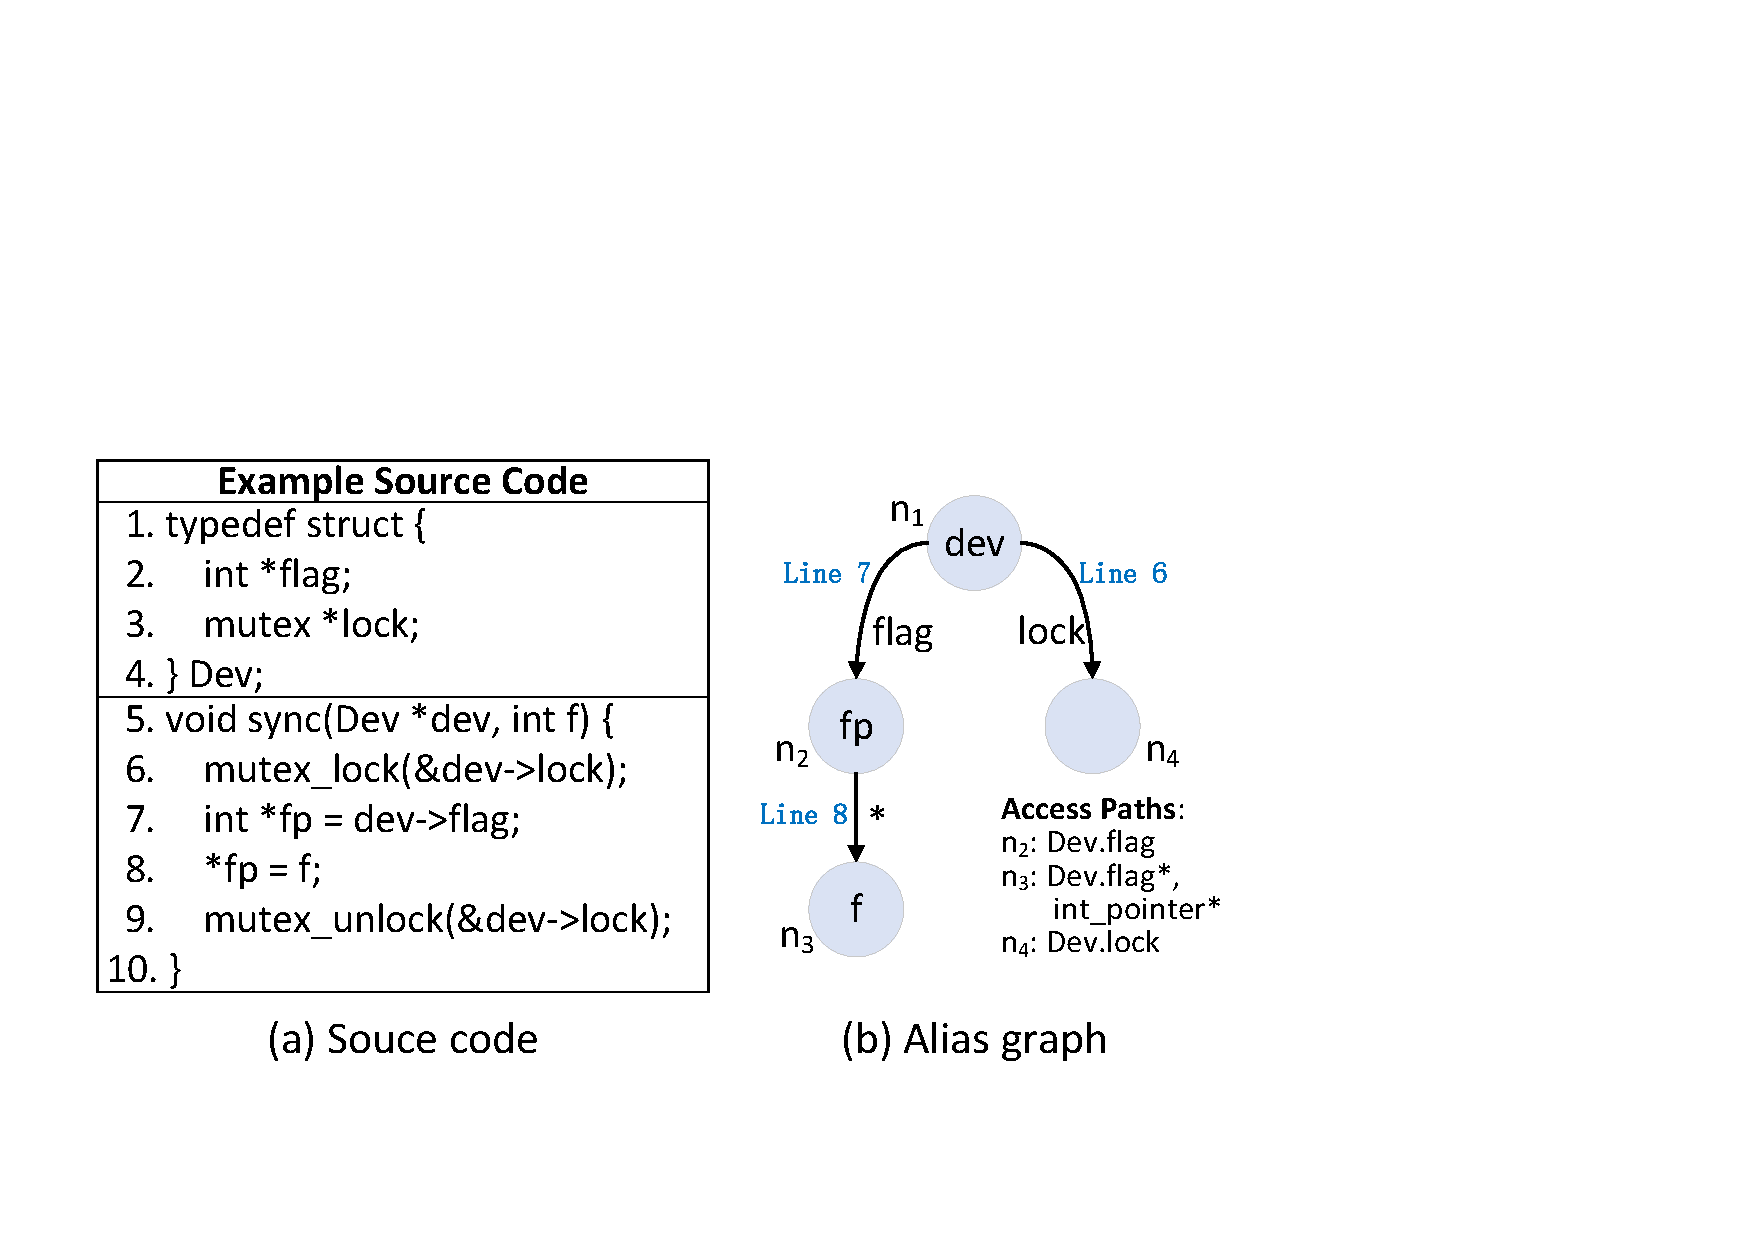
\includegraphics[width=0.9\linewidth]{figures/fig_alias_graph_demo.pdf}
	\figcaption{Example of alias graph.}
	\label{fig_alias_graph_demo}
\end{figure}

\noindent{\textbf{\em Example.}} Figure~\ref{fig_alias_graph_demo} shows a 
piece of driver-like source code and its alias graph. In this example, after an 
GEP (\&dev->lock) operation at Line 6, an edge labeled with {\tt lock} from 
node $\mathit{n_1}$ to node $\mathit{n_4}$ is inserted. Similarly, an edge 
labeled with {\tt flag} from node $\mathit{n_1}$ to node $\mathit{n_2}$ is 
inserted after Line 7. At last, an edge labeled with a dereference operator 
($\mathit{*}$) is inserted after the STORE (*fp = f) operation at Line 8. The 
final alias graph is shown in Figure~\ref{fig_alias_graph_demo}(b), and access 
paths are shown in the bottom left corner. Take node $\mathit{n_3}$ as an 
example, it can represent two fields, one is {\tt Dev.flag*}, and the other is 
{\tt int\_pointer*} (we exploit int\_pointer to represent a pointer points to 
an integer, and regard it as a data structure for convenience). 

\begin{figure}[htbp]
	\centering
	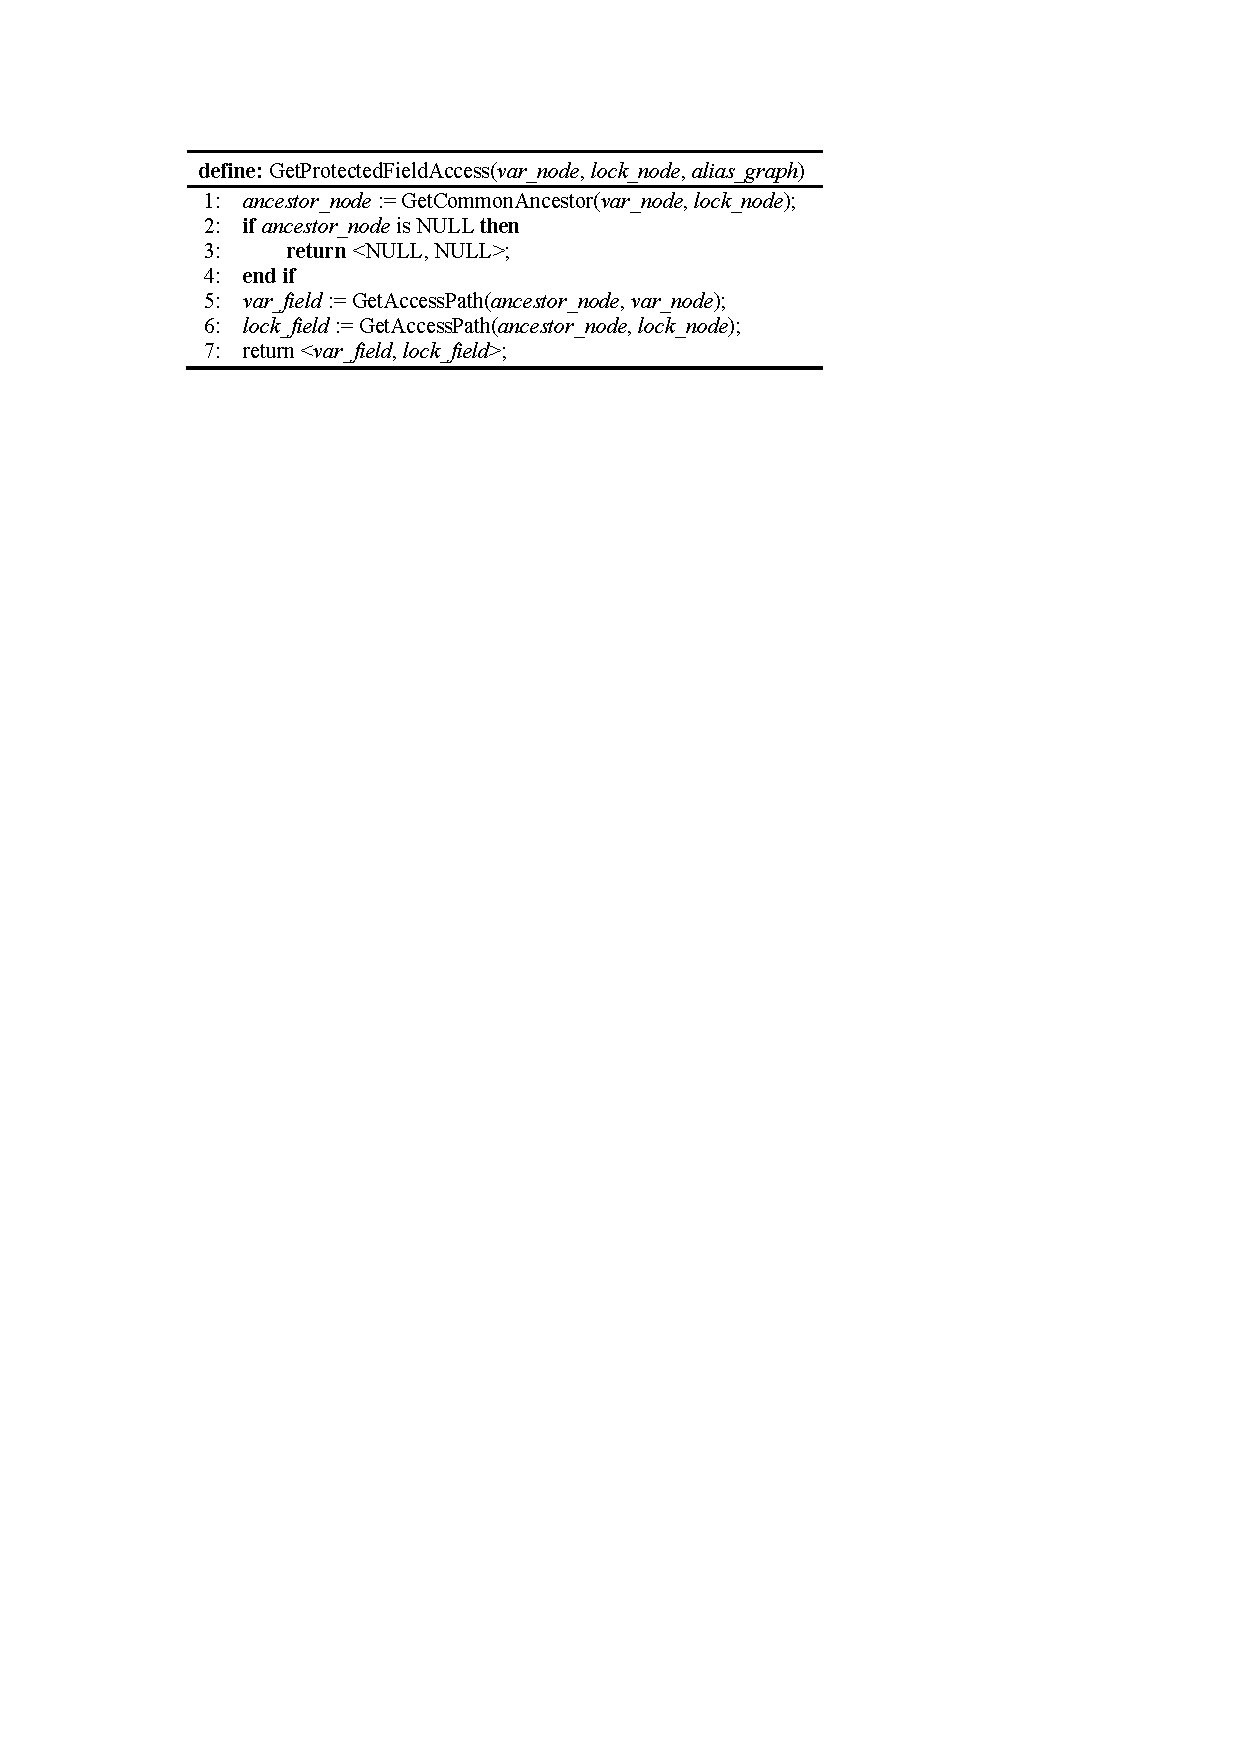
\includegraphics[width=1\linewidth]{figures/fig_pseudocode_get_access.pdf}
	\figcaption{Pseudocodes to get accessed field and protecting lock.}
	\label{fig_pseudocode_get_access}
\end{figure}

Given an alias graph, whether a variable and a lock exist in the same data 
structure can be determined by finding a common ancestor. If they are in the 
same data structure, the lock is likely to protect the variable when it is 
accessed. Figure~\ref{fig_pseudocode_get_access} shows the pseudocode to 
get the field of the accessed variable and the field of the protecting lock in 
the form of access path, if they exist in the same data structure. Given a node 
of an accessed variable and a node of a lock variable, the analysis first gets 
the common ancestor of the two nodes (Line 1). And then, if the common ancestor 
does not exist, the analysis returns NULL (Lines 2-3). Otherwise, the analysis 
gets the access path for the node of the accessed variable and the node of the 
lock variable from the common ancestor (Lines 5-7).

%\begin{table}[htbp]
%	\tablecaption{Notation table of pseudocodes.}
%	\label{tbl_notation}
%	\centering
%	\scriptsize
%	\begin{spacing}{0.98}
%		\begin{tabular}{@{ }p{2.7cm}p{5.05cm}@{ }}
%		\toprule[1pt]
%		GetAliasNode($\mathit{var}$, $\mathit{alias\_graph}$) & Get the node 
%		the variable $\mathit{var}$ exists in from the alias graph 
%		$\mathit{alias\_graph}$. \\ \hline
%		GetCommonAncestor($\mathit{node_1}$, $\mathit{node_2}$) & Get the 
%		common ancestor of the two nodes $\mathit{node_1}$ and 
%		$\mathit{node_2}$. \\ \hline
%		GetAccessPath($\mathit{node_1}$, $\mathit{node_2}$) & Get the access 
%		path from $\mathit{node_1}$ to $\mathit{node_2}$ \\ \hline
%		\bottomrule[1pt]	
%		\end{tabular}
%	\end{spacing}
%\end{table}

Take the alias graph in Figure~\ref{fig_alias_graph_demo} as an example, {\tt 
\&dev->flag} is represented by node $\mathit{n_2}$, and {\tt \&dev->lock} is 
represented by node $\mathit{n_4}$. The two nodes have a common ancestor 
$\mathit{n_1}$, and thus the accessed variable {\tt \&dev->flag} and the 
protecting lock {\tt \&dev->lock} can be inferred to exist in the same data 
structure (namely {\tt Dev}). Therefore, the structure field Dev.flag is likely 
to be protected the lock stored in the structure field Dev.lock.

\begin{figure}[htbp]
	\centering
	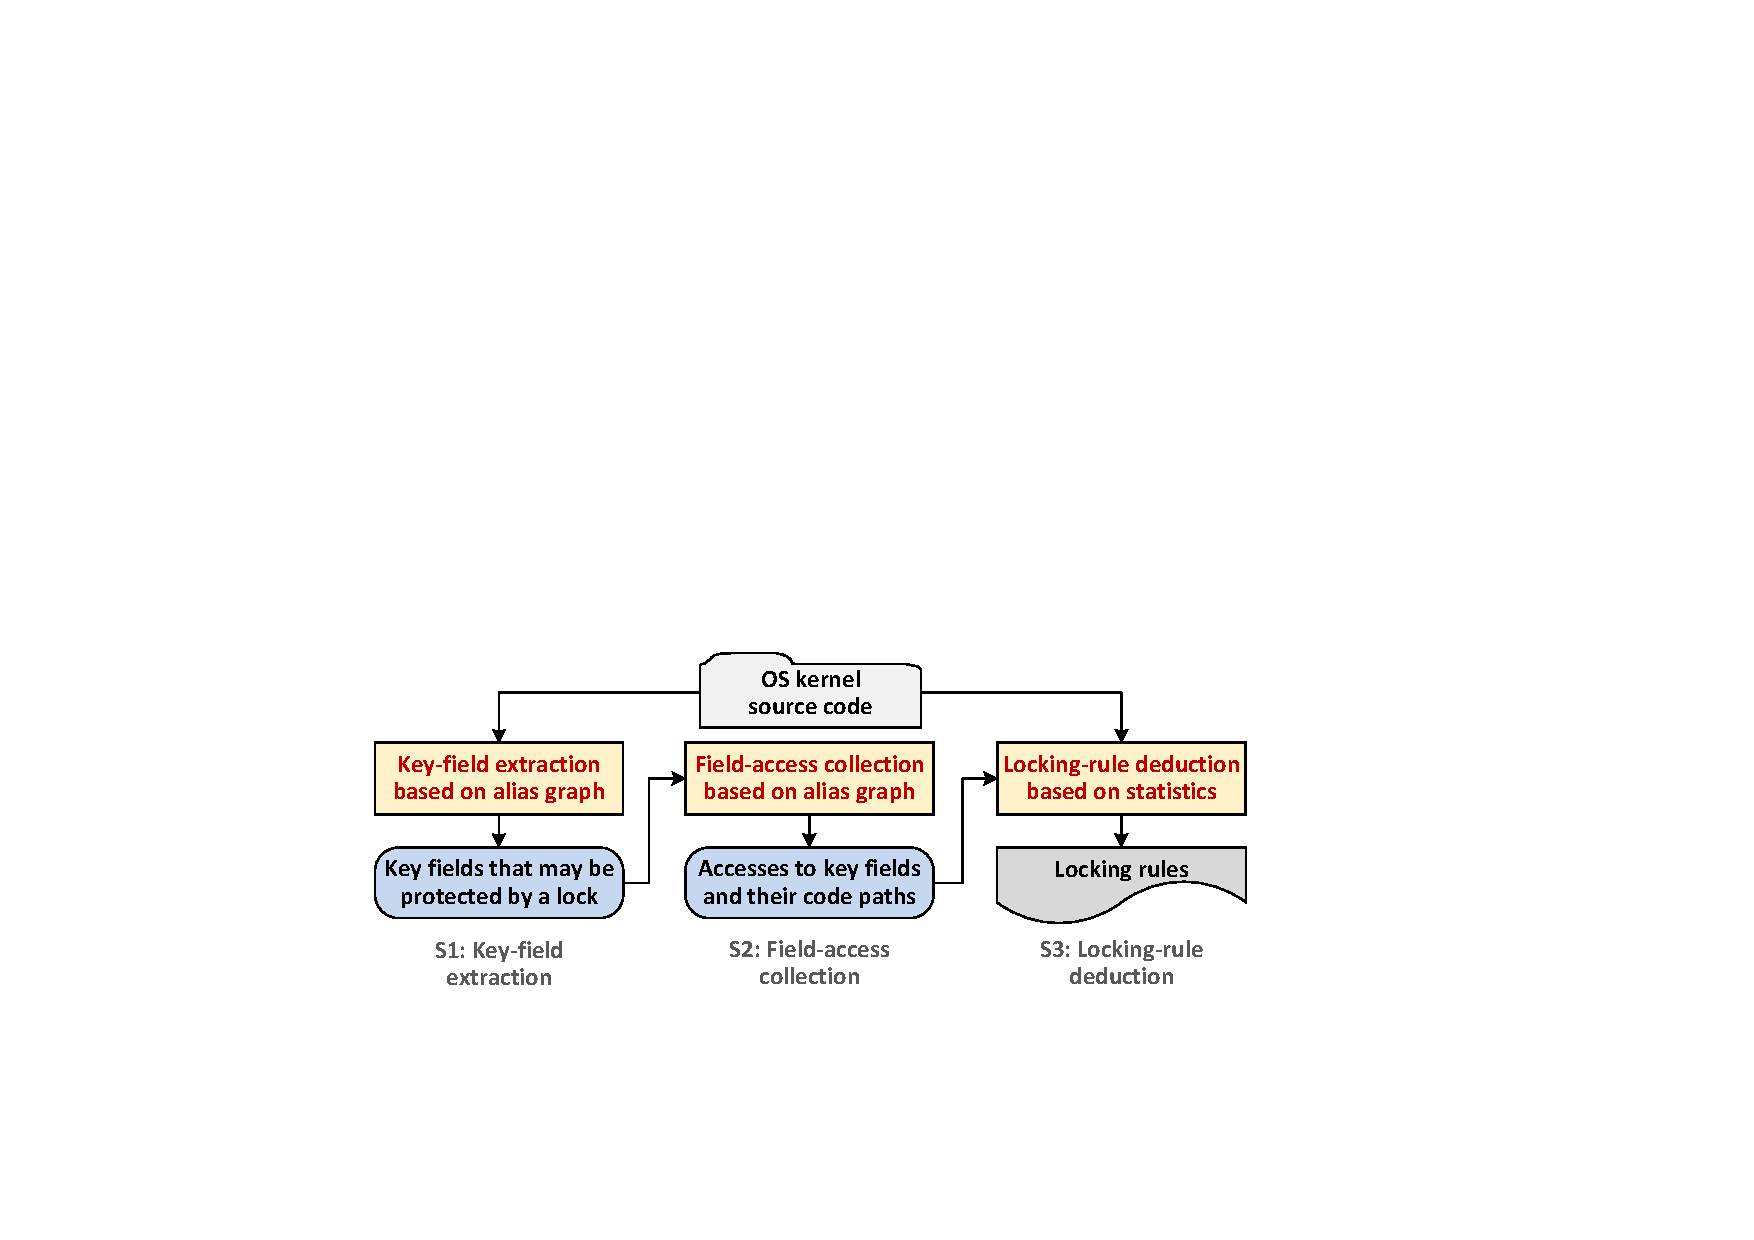
\includegraphics[width=1\linewidth]{figures/fig_workflow.pdf}
	\figcaption{Workflow of locking-rule mining.}
	\label{fig_workflow}
\end{figure}

Based on the alias graph, our alias-aware rule mining method performs an 
inter-procedural path-based~\cite{Li:ASPLOS22}, field-sensitive and alias-aware 
analysis to effectively mine locking rules about whether a specific variable 
should be protected by a lock and which lock is required. Overall, our 
alias-aware rule mining method has three main stages shown in 
Figure~\ref{fig_workflow}. In Stage 1, it extract key variable that may be 
protected by a lock. In Stage 2, it collect all accesses to key fields as well 
as code paths these accesses exist in. In Stage 3, it deduce locking rules by 
calculate the proportion of field accesses protected by a specific lock in all 
field accesses. 

\PP{S1: Key-field Extraction.} The OS Kernel has a large code base with 
numerous variables. However, only a small part of variables should be protected 
by a specific lock, and thus collecting all variable accesses can introduce 
much unnecessary overhead. Generally, only a few field accesses can miss 
necessary protecting lock, due to carelessness of developers. Based on this 
insight, our analysis first extracts key fields that may need to be protected 
by a specific lock, by performing a lock-set analysis to find whether a given 
variable is accessed after acquiring a lock in the same data structure as the 
accessed field in any code path.

\begin{figure}[htbp]
	\centering
	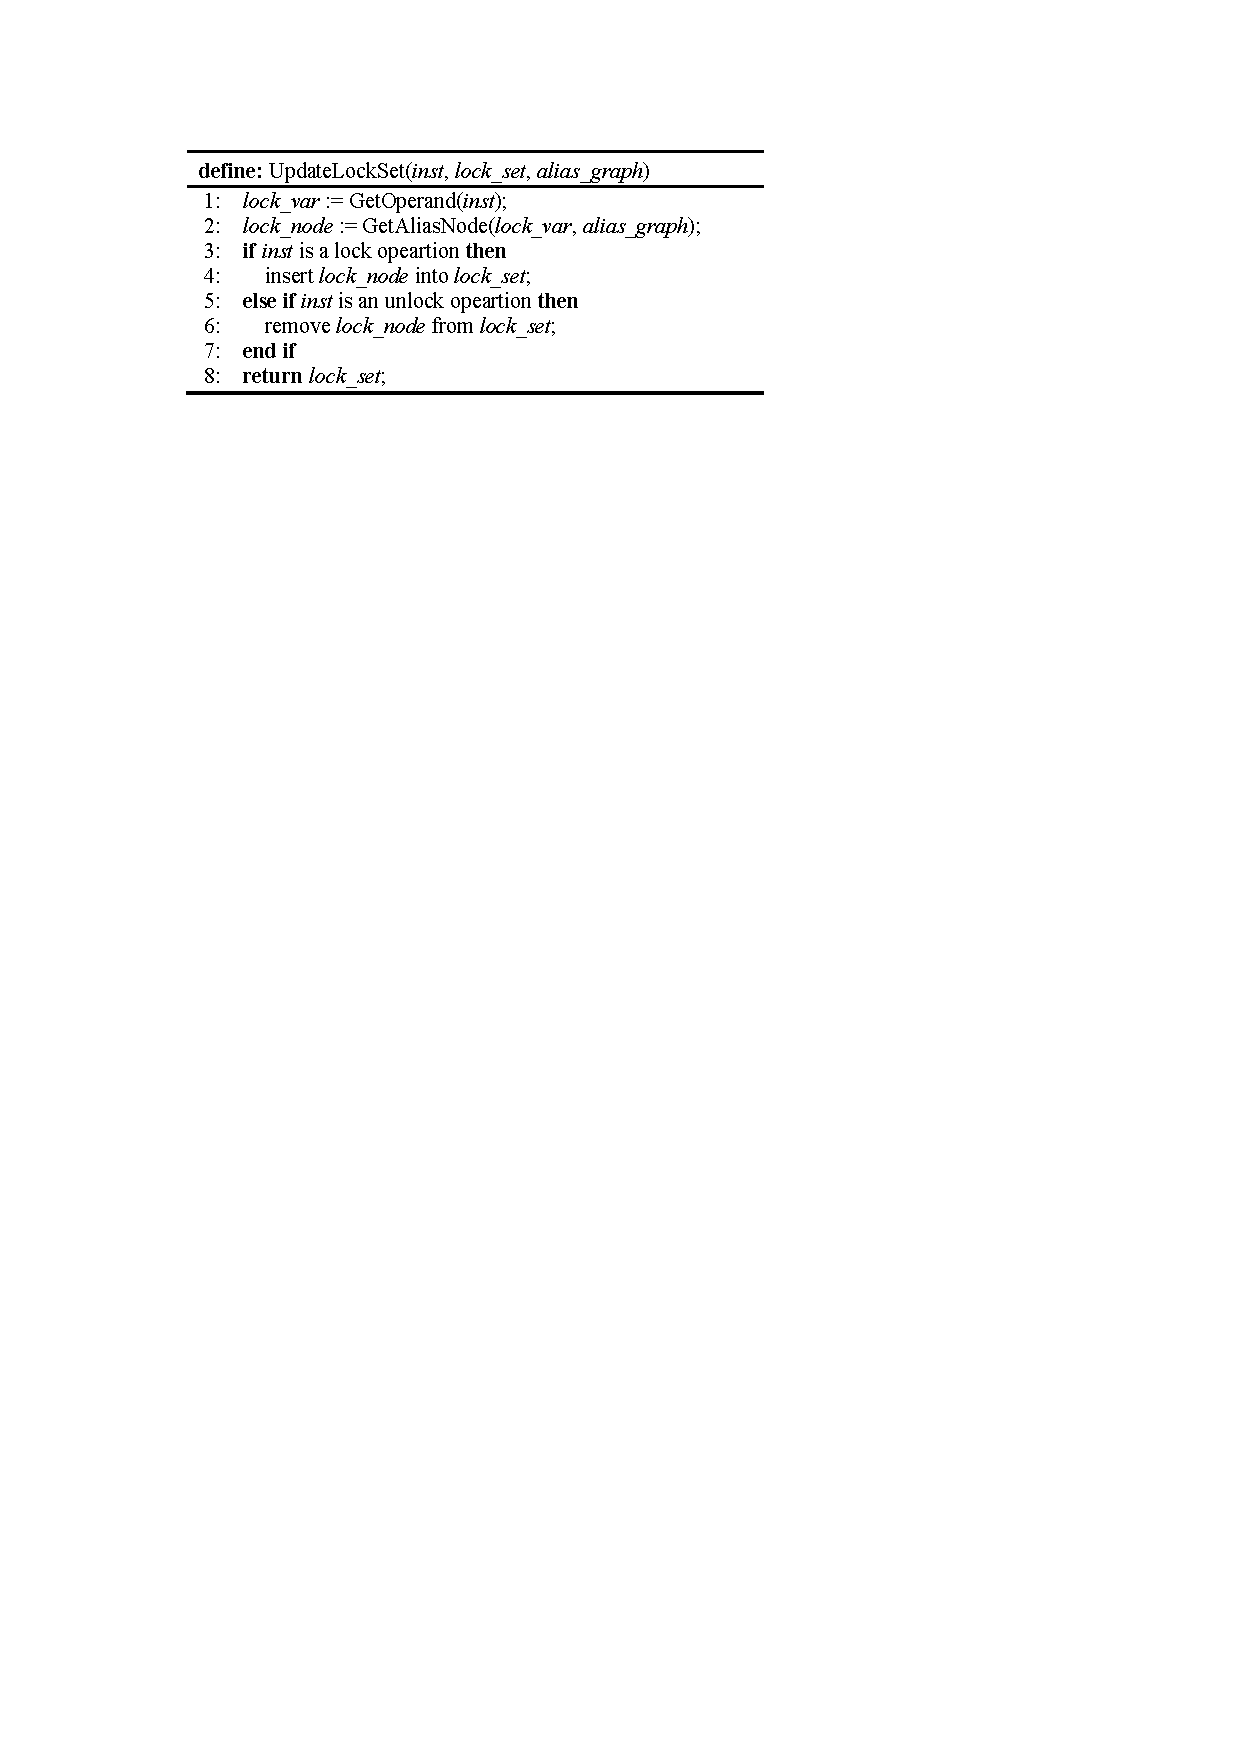
\includegraphics[width=0.9\linewidth]{figures/fig_pseudocode_lock_set.pdf}
	\figcaption{Pseudocodes of lock-set analysis.}
	\label{fig_pseudocode_lock_set}
\end{figure}

Figure~\ref{fig_pseudocode_lock_set} shows the lock-set analysis based on alias 
graph. The analysis first gets the operand of the instruction (Line 1), and 
then get the node of the operand from the alias graph (Line 2). If the 
instruction is a lock operation, the node of the operand is inserted into the 
lock set (Lines 3-4). Otherwise, if the instruction is an unlock operation, the 
node of the operand is removed from the lock set (Lines 5-6).

\begin{figure}[htbp]
	\centering
	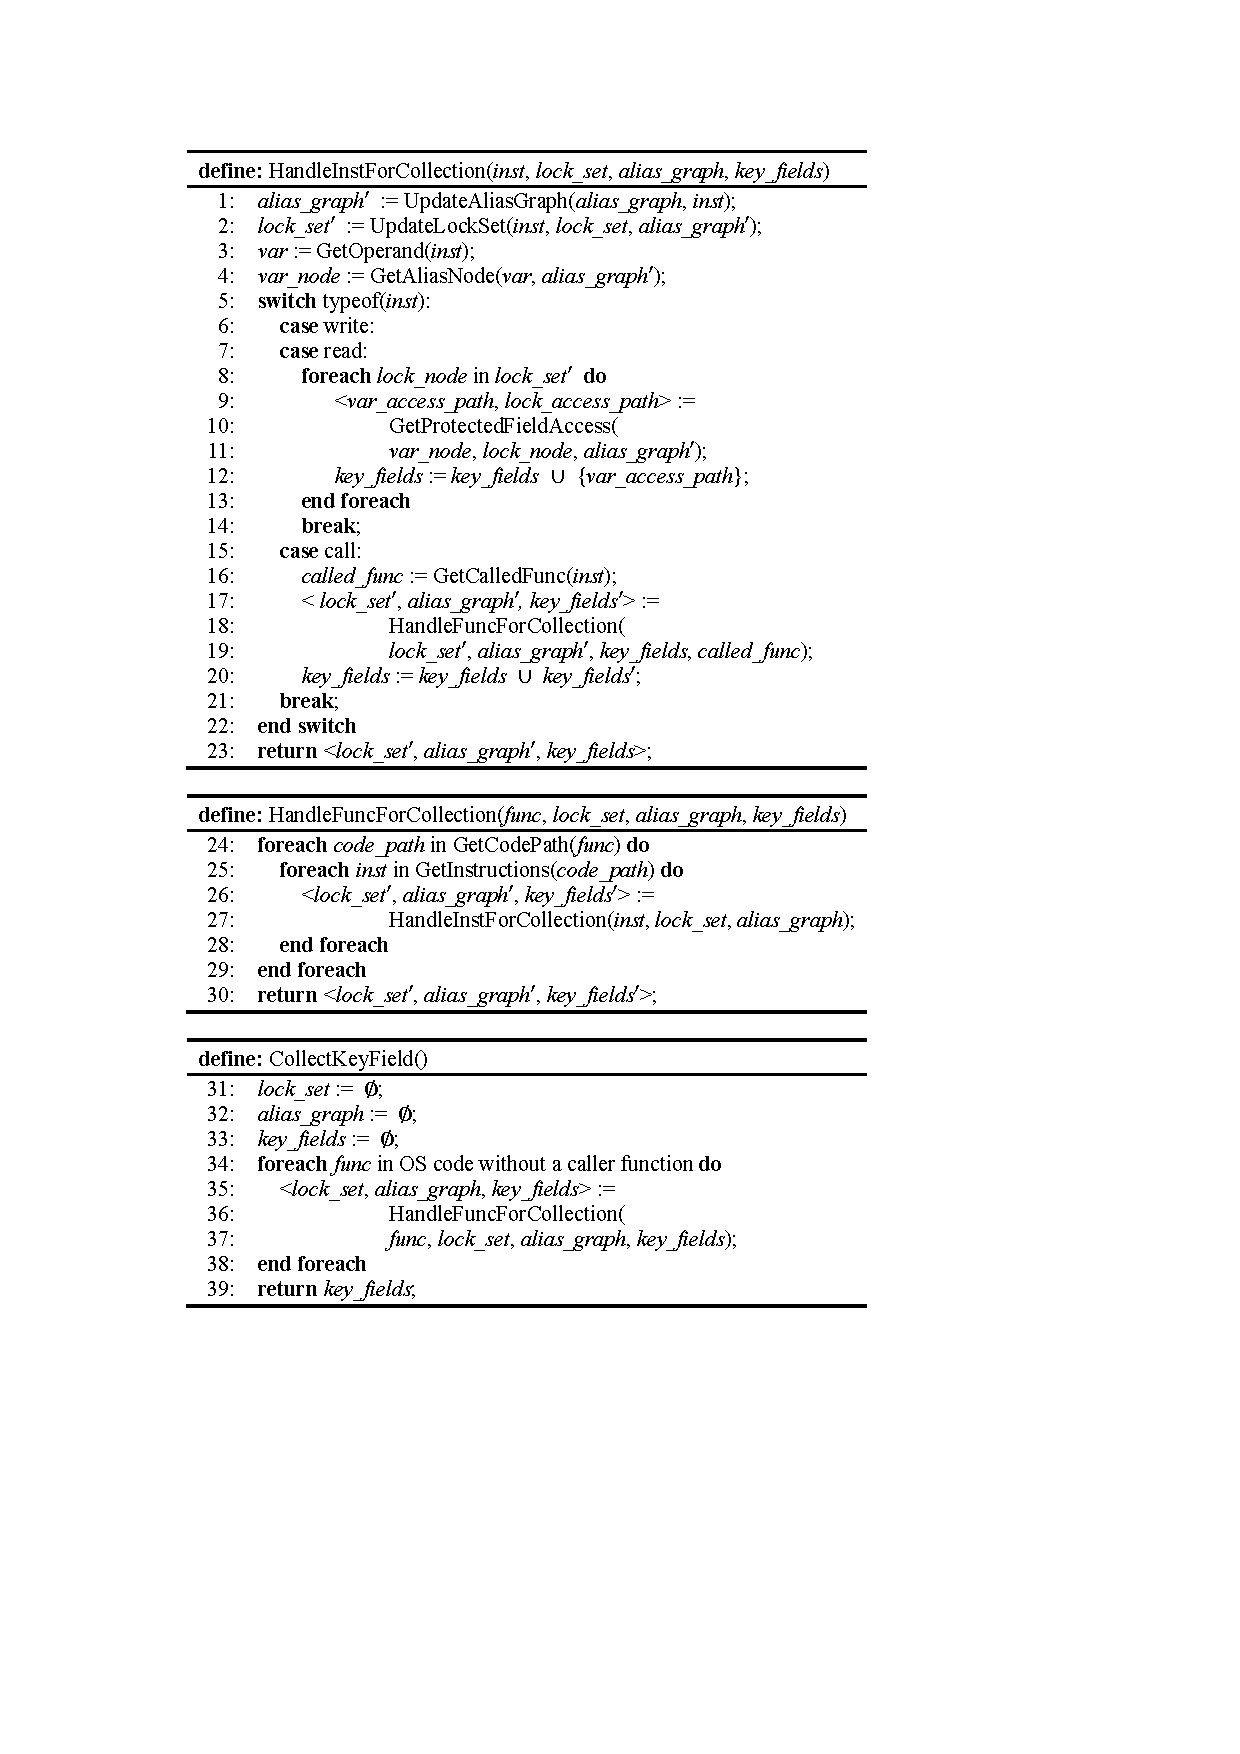
\includegraphics[width=1\linewidth]{figures/fig_pseudocode_field_extract.pdf}
	\figcaption{Pseudocodes of key-field extraction.}
	\label{fig_pseudocode_field_extract}
\end{figure}

Figure~\ref{fig_pseudocode_field_extract} shows the pseudocode to collect key 
fields that may be protected by a specific lock when are accessed, based on 
lock-set analysis and alias graph. The analysis start analyzing 

For each function without a caller function, the analysis 

